% =============================================================
%  MAIN REPORT TEMPLATE
%  Compile this file to produce the full report.
%  Each section lives in its own file under sections/
% =============================================================

\documentclass[12pt, letterpaper]{book}

% ----- Packages -----------------------------------------------
\usepackage[T1]{fontenc}
\usepackage[utf8]{inputenc}
\usepackage{lmodern}              % Improved font rendering
\usepackage[margin=1in]{geometry} % Page margins
\usepackage{setspace}             % Line spacing
\usepackage{parskip}              % Space between paragraphs
\usepackage{titlesec}             % Section title formatting
\usepackage{fancyhdr}             % Headers and footers
\usepackage{graphicx}             % Figures
\usepackage{booktabs}             % Professional tables
\usepackage{caption}              % Caption formatting
\usepackage{hyperref}             % Clickable TOC & cross-references
\usepackage{cleveref}             % Smart cross-references
\usepackage{natbib}               % Bibliography (author-year style)
\usepackage{appendix}             % Appendix formatting
\usepackage{lipsum}               % Placeholder text — remove when done
\usepackage{siunitx}              % SI units formatting

% ----- Hyperref setup -----------------------------------------
\hypersetup{
    colorlinks  = true,
    linkcolor   = blue,
    citecolor   = green,
    urlcolor    = blue,
    pdftitle    = {Project Report},
    pdfauthor   = {Author Name},
}

% ----- Page style ---------------------------------------------
\pagestyle{fancy}
\fancyhf{}
\fancyhead[L]{\small\leftmark}
\fancyhead[R]{\small\thepage}
\fancyfoot[C]{\small\textit{Project Report}}
\renewcommand{\headrulewidth}{0.4pt}

% ----- Section title formatting -------------------------------
\titleformat{\chapter}[display]
    {\normalfont\Large\bfseries}{\chaptertitlename\ \thechapter}{10pt}{\Huge}
\titlespacing*{\chapter}{0pt}{-20pt}{20pt}

% ----- Line spacing -------------------------------------------
\onehalfspacing

% =============================================================
%  DOCUMENT BODY
% =============================================================
\begin{document}

% ----- Title Page ---------------------------------------------
% =============================================================
%  TITLE PAGE  (sections/00_titlepage.tex)
% =============================================================

\begin{titlepage}
    \centering
    \vspace*{2cm}

    % Institution / Course
    {\large\textbf{Course / Institution Name}\\[0.3cm]}
    {\large Course Number \& Title\\[2cm]}

    % Report title
    {\Huge\bfseries Project Report Title\\[0.5cm]}
    {\large\itshape Subtitle (if applicable)\\[2.5cm]}

    % Authors
    \begin{tabular}{c}
        \textbf{Author One} \\
        \textbf{Author Two} \\
        \textbf{Author Three} \\
    \end{tabular}\\[2cm]

    % Date
    {\large \today}

    \vfill

    % Supervisor / Instructor (optional)
    {\normalsize Submitted to: Professor Name\\}
    {\normalsize Department Name}
\end{titlepage}


% ----- Front matter (roman numerals) --------------------------
\frontmatter

% Executive Summary (unnumbered, appears before TOC)
% =============================================================
%  EXECUTIVE SUMMARY  (sections/01_executive_summary.tex)
% =============================================================

% =============================================================
%  EXECUTIVE SUMMARY  (sections/01_executive_summary.tex)
% =============================================================

\chapter*{Executive Summary}
\addcontentsline{toc}{chapter}{Executive Summary}
\markboth{Executive Summary}{Executive Summary}

This report presents the well design, surface network configuration, pipeline sizing, economic analysis, and production strategy for a subsea field development project comprising seven production wells. The work was carried out in two parts: a PIPESIM-based study and the development of an in-house Python network simulator.

\textbf{Well Design.} Each well was designed to deliver a maximum liquid rate of 6{,}429~STB/d, corresponding to a field target of 45{,}000~STB/d. A productivity-index analysis identified a 7-inch OD (5.92-inch ID) production casing as the optimal selection, balancing inflow performance against drilling cost. The minimum tubing ID of 2.922 inches (3.5-inch OD) was determined from PIPESIM wellbore simulations. Gas-lift is required at water cuts above 5\%, with a maximum injection rate of 1.6~MMscf/d per well at 95\% water cut. A minimum wellhead pressure of 1{,}200~psia is maintained throughout, preventing asphaltene precipitation.

\textbf{Pipeline Design.} The subsea flowline connecting manifold M2 to the land-based operations point (LOP) is 46{,}617~ft long with a maximum riser depth of 3{,}000~ft. A 10-inch internal diameter was selected as the minimum viable size, yielding an inlet pressure of 1{,}040~psia at worst-case conditions (WC~=~2\%, 7~wells), within the 1{,}200~psia constraint. The system remains operable with four wells online. Thermal analysis confirmed that a minimum insulation thickness of 2~inches is required to keep outlet temperatures above the wax appearance temperature of 100\textdegree F under reduced-production conditions.

\textbf{Economic Analysis and Production Optimization.} A gas-lift optimization algorithm was applied to maximize net profit over the production forecast. At \$50/BBL, optimized gas-lift scheduling sustains economic production across the full forecast period, compared to an economic limit at day~14{,}512 without optimization. At \$30/BBL, optimization extends economic production by approximately 10{,}015~days. Break-even water cuts were estimated at 86\% and 78\% for oil prices of \$50/BBL and \$30/BBL, respectively.

\textbf{Network Simulator.} An integrated Python network simulator was developed, coupling subsurface inflow models with surface multiphase flow using the Hagedorn--Brown (wellbore) and Beggs--Brill (pipeline) correlations. Simulation results showed good agreement with PIPESIM, demonstrating the tool's utility for production optimization when commercial software is unavailable.

% Table of Contents
\tableofcontents
\listoffigures          % Remove if no figures
\listoftables           % Remove if no tables
\newpage

% ----- Main matter (arabic numerals) --------------------------
\mainmatter

% =============================================================
%  INTRODUCTION  (sections/02_introduction.tex)
% =============================================================

\chapter{Introduction}

% Brief description of the project and its objectives.
% Provide context: background, motivation, and scope of work.
% Refer the reader to the Appendix for the full project description.

\lipsum[3] % Replace with your introduction text

The complete project description, as issued in the course handout,
is reproduced in \cref{app:project_description}.

% =============================================================
%  PROCEDURE  (sections/03_procedure.tex)
% =============================================================

\chapter{Procedure}

% Describe WHAT YOU DID in enough detail that someone else could
% replicate the work. Use subsections to organise distinct phases
% or methods. Keep subsection names consistent with those you will
% use in the Results chapter.

% ----- Subsection 1 -------------------------------------------
\section{Part 1}
\label{sec:proc_part1}
\subsection{Well Design}
This subsecion describes the design of the default well. Because the wells were not drilled, it is necessary to specify the tubing and production casing.
Is was informed that the inflow can be modeled as a single-phase steady-state solution of the Darcy equation for a vertical fully penetrating well.
The Productivity Index (PI) equation is given by:
\begin{equation}
    PI = \frac{q_{liq}}{\bar{p} - p_{wf}} = \frac{kh}{141.2 B_o \mu_o \left[\ln{\left(\frac{r_e}{r_{wf}}\right)}-0.5 + S\right]} \quad \text{STB/d/psi}
\end{equation}
Where $q_{liq}$ is the liquid flow rate in STB/d, $\bar{p}$ is the average reservoir pressure, $p_{wf}$ is the bottom hole flowing pressure (psi), $k$ is the permeability in mD, $h$ is the thickness of the reservoir in ft, $B_o$ is the oil formation volume factor (RB/STB), $\mu_o$ is the oil viscosity (cP), $r_e$ is the drainage radius (ft), $r_{wf}$ is the wellbore radius (ft) and $S$ is the skin factor.
The reservoir properties are given in Table \ref{tab:reservoir_properties}.

% =============================================================
%  RESERVOIR & FLUID PROPERTIES TABLE
%  Drop this block into any section file, e.g. 03_procedure.tex
%  Requires: booktabs, siunitx (add to main.tex preamble)
% =============================================================

% Add to main.tex preamble if not already present:
% \usepackage{booktabs}
% \usepackage{siunitx}

\begin{table}[htbp]
    \centering
    \caption{Reservoir and Fluid Properties}
    \label{tab:reservoir_properties}
    \begin{tabular}{l l r l}
        \toprule
        \textbf{Parameter} & \textbf{Symbol} & \textbf{Value} & \textbf{Unit} \\
        \midrule
        \multicolumn{4}{l}{\textit{Reservoir Conditions}} \\
        \midrule
        Reservoir pressure       & $\bar{P}$  & 3800          & psia          \\
        Reservoir temperature    & $T$         & 200           & $^\circ$F     \\
        \midrule
        \multicolumn{4}{l}{\textit{Rock Properties}} \\
        \midrule
        Permeability             & $k$         & 40            & mDarcy        \\
        Net pay thickness        & $h$         & 150           & ft            \\
        Drainage radius          & $r_e$       & 372           & ft            \\
        Skin factor              & $S$         & 0             & --            \\
        \midrule
        \multicolumn{4}{l}{\textit{Fluid Properties}} \\
        \midrule
        API gravity              & API         & 45            & $^\circ$API   \\
        Oil viscosity (res.)     & $\mu_o$     & 0.902         & cp            \\
        Gas specific gravity     & $\gamma_g$  & 0.6636        & --            \\
        Gas-oil ratio            & GOR         & 800           & scf/STB       \\
        Bubble point pressure    & $P_b$       & 3800          & psia @ 200$^\circ$F \\
        Formation volume factor  & $B_o$       & 1.2           & RB/STB @ $P_b$ \\
        \midrule
        \multicolumn{4}{l}{\textit{Production Constraints}} \\
        Maximum rroduction rate & $q_{\max}$   & 45,000        & STB/d         \\
        Number of production wells          & $N_{wells}$   & 7             & --            \\
        Minimum wellhead pressure & $P_{wh,\min}$  & 1200          & psia          \\
        \bottomrule
    \end{tabular}
\end{table}

It was stated that the drilling and completion costs are highly sensitive to the wellbore radius ($r_{wf}$). So, first, we should
try to finde the minimum tubing size that allows to produce the maximum flow rate for each development scenario. The maximum flow rate per well 
was defined as $q_{\max} / N_{wells}$, which is 6428.57 STB/d. The Figure \ref{fig:pi_x_radii} shows the relationship between the Productivity Index and the wellbore radius for the given reservoir and fluid properties.
From the plot, it is observed that the PI range is between 5.5 and 6.0 STB/d/psi for a casing OD between 4.5 and 7.75 inches (9\% improvement) but the difference between the 7 and 7.75 inches is only 0.1 STB/d/psi (1.7\% improvement). 
\begin{figure}[htbp]
    \centering
    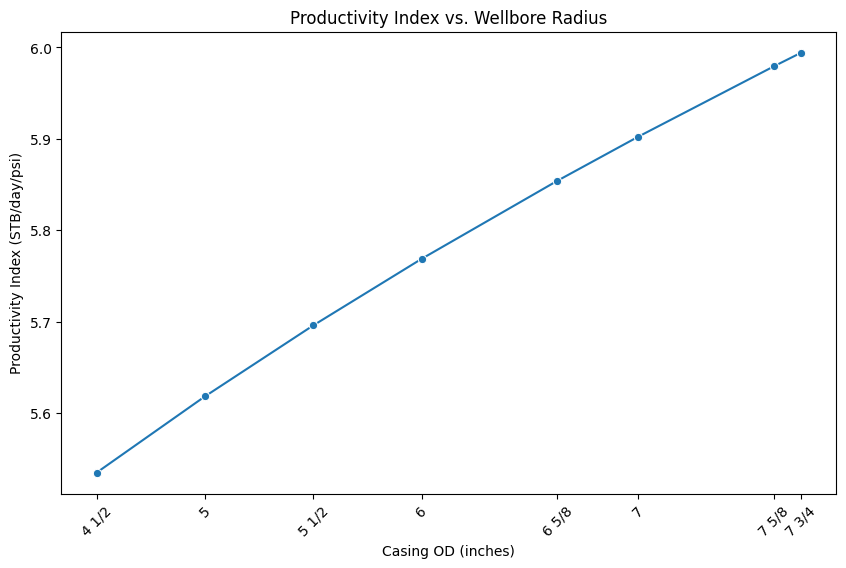
\includegraphics[width=0.7\textwidth]{figs/pi_vs_radius.png}
    \caption{Productivity Index vs. Wellbore Radius}
    \label{fig:pi_x_radii}
\end{figure}
It was also assumed that the tubing size should be $0.8 r_{wf}$. The behaviour of the Producivity Index is shown in Figure \ref{fig:pi_x_tubing_radius}. Because the PI is just a function of the wellbore radius, the plot is the same as in Figure \ref{fig:pi_x_radii}, but with a different x-axis. 
\begin{figure}[htbp]
    \centering
    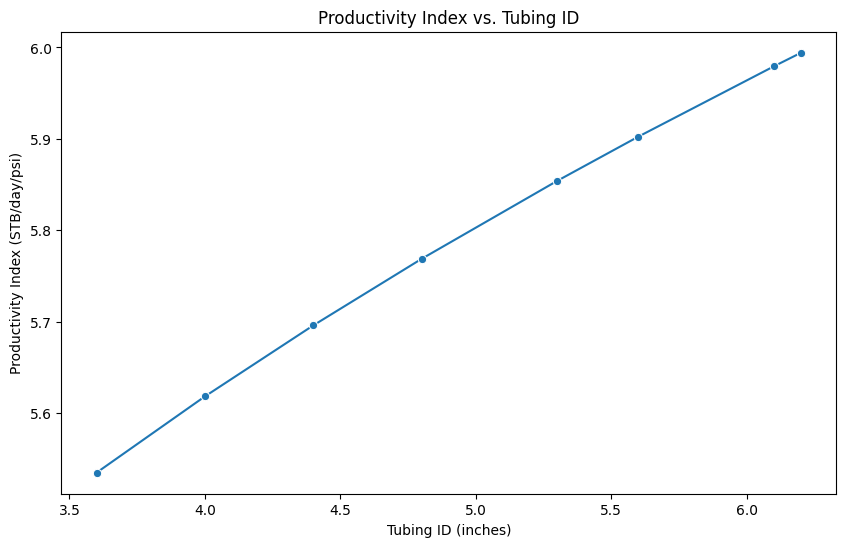
\includegraphics[width=0.7\textwidth]{figs/pi_vs_tubing_radius.png}
    \caption{Productivity Index vs. Tubing Radius}
    \label{fig:pi_x_tubing_radius}
\end{figure}

It was adivised that the asphaltene precipitation occurs at a pressure of 1100 psis, so the minimum wellhead pressure should be at least 1200 psia. 
A wellbore model of Well 1 was created using Pipesim and the impact of tubing ID was evaluated. The results are shown in Figure \ref{fig:well1_q_x_tubing_radius}. It can be observed that the flow rate is higher than the maximum allowed for all tubing sizes, but the 4.5 inches tubing has a flow rate of 7000 STB/d, which is much higher than the maximum allowed. The 7 inches tubing has a flow rate of 6500 STB/d, which is also higher than the maximum allowed but closer to it. The 7.75 inches tubing has a flow rate of 6400 STB/d, which is just below the maximum allowed. Therefore, the 7 inches tubing was selected for Well 1.
\begin{figure}[htbp]
    \centering
    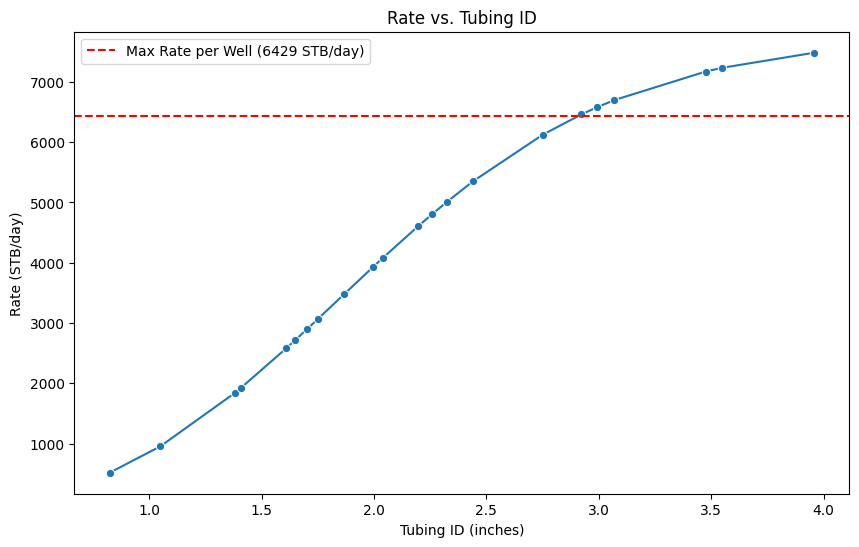
\includegraphics[width=0.7\textwidth]{figs/rate_vs_tubing_id.png}
    \caption{Flow Rate vs. Tubing Radius for Well 1}
    \label{fig:well1_q_x_tubing_radius}
\end{figure}
The minimum tubing ID that allows to produce the maximum flow rate was 2.922 inches, which corresponds to a tubing OD of 3.5 inches. Because it is necessary to have as least 1 inch of annular space between the tubing and the casing, the minimum casing ID should be 5.5 inches. 
A 5.5 ID casing corresponds to a 6.625 inches OD casing. In our project, we decided to use a 7 inches OD casing due to the best productivity index and the fact that it is a common casing size. A larger casing size would not be justified because the improvement in the productivity index is not significant and it would increase the drilling and completion costs.
The production forecast predicts the water cut will improve and it was necessary to evaluate the impact of water cut on the flow rate. The results are shown in Figure \ref{fig:well1_q_x_water_cut}. It can be observed that the well rate does not produce the maximum allowed flow rate for a water cut higher than 10\%. 
\begin{figure}[htbp]
    \centering
    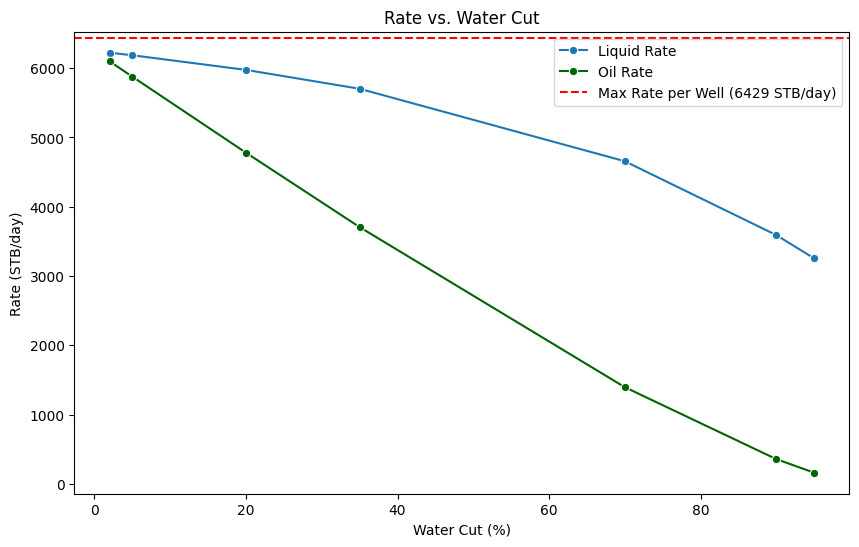
\includegraphics[width=0.7\textwidth]{figs/rate_vs_watercut.png}
    \caption{Flow Rate vs. Water Cut for Well 1}
    \label{fig:well1_q_x_water_cut}
\end{figure}
So, it was observed that when the well starts to produce water, the maximum liquid rate is not achieved, so it is necessary to implement artificial lift. 
The only artificial lift option available is the gas-lift. The gas-lift rate was evaluated for different water cuts and the results are shown in Figure \ref{fig:well1_gas_lift_rate_x_water_cut}. 
It is observed that the minimum gas-lift rate that allows to produce the maximum liquid rate for all water cuts is 1.5 MMscf/d. 
\begin{figure}[htbp]
    \centering
    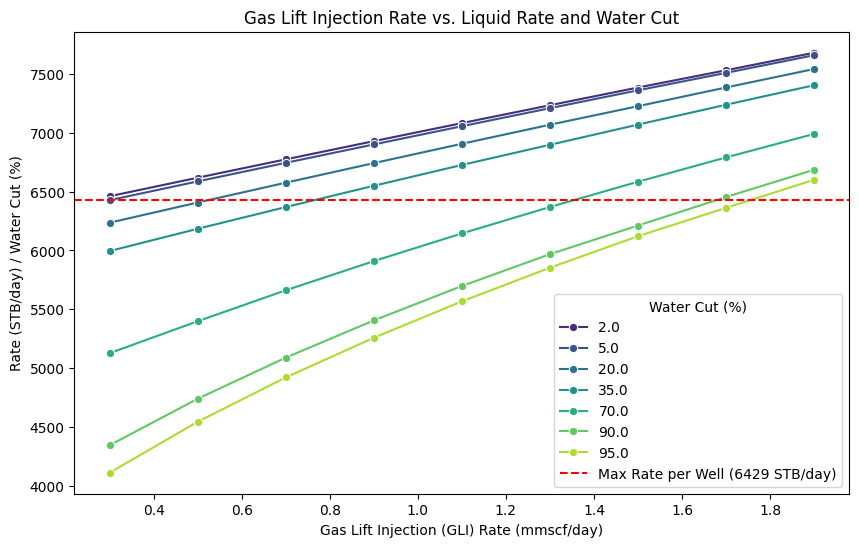
\includegraphics[width=0.7\textwidth]{figs/rate_vs_gas_lift.png}
    \caption{Gas-Lift Rate and Water Cut vs. Liquid Rate for Well 1}
    \label{fig:well1_gas_lift_rate_x_water_cut}
\end{figure}
% ----- Subsection 2 -------------------------------------------
\section{Part 2}
\label{sec:proc_phase2}
It was also analyzed the impact of the gas-lift rate and water cut on the wellhead temperature. The results are shown in Figure \ref{fig:well1_q_x_gas_lift_and_temp}. 
It was not informed the minimum wellhead temperature, but for this configuration, the wellhead temperature is above 176$^\circ$F for all water cuts and gas-lift rates.
\begin{figure}[htbp]
    \centering
    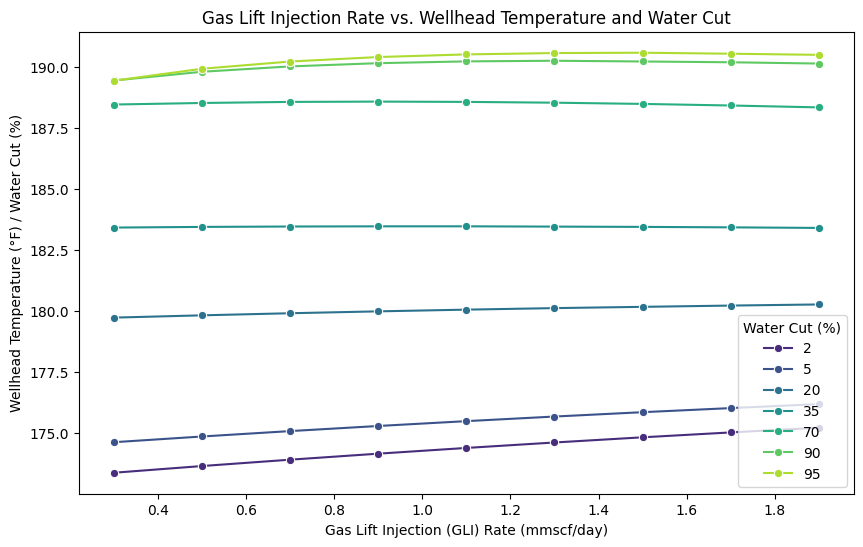
\includegraphics[width=0.7\textwidth]{figs/rate_vs_gas_lift_and_temp.png}
    \caption{Wellhead Temperature vs. Gas-Lift Rate and Water Cut for Well 1}
    \label{fig:well1_q_x_gas_lift_and_temp}
\end{figure}


\lipsum[6] % Replace with description of second method / phase

% Add or remove \section{} blocks as needed.

% =============================================================
%  RESULTS  (sections/04_results.tex)
% =============================================================

\chapter{Final Network Configuration and Production Strategy}

% Present your results using the SAME subsection structure as the
% Procedure chapter. Reference figures and tables in the text;
% do not let them stand alone without discussion.

% ----- Subsection 1 -------------------------------------------
\section{Wells}
\label{sec:res_wells}
The well design process was developed as shown in Section~\ref{subsec:well}. It was defined the tubing and production casing for the default well. 
It was also informed the gas lift rate needed to mantain the production rate of 6428.57 bbl/day. The final design of the well is shown in Table~\ref{tab:well_design}.
\begin{table}[ht]
    \centering
    \caption{Final well design.}
    \label{tab:well_design}
    \begin{tabular}{lccc}
        \hline
        Parameter & OD & ID & Unit \\
        \hline
        Tubing Diameter & 3.5 & 2.922 & inches \\
        Production Casing Diameter & 7.0 & 5.92 & inches \\
        \hline
    \end{tabular}
\end{table}

The gas lift is need for water cuts higher than 5\%. The maximum gas lift rate needed is 1.6~MMscf/day, for a water cut of 95\%. The Table~\ref{tab:gas_lift} shows the minimum gas lift rate needed for different water cuts.
Using those gas lift rates is also asured that the well head pressure will be higher than 1200 psi, which is the minimum pressure needed to avoid parafin deposition.
\begin{table}[ht]
    \centering
    \caption{Minimum gas lift rate needed for different water cuts.}
    \label{tab:gas_lift}
    \begin{tabular}{lcc}
        \hline
        Water Cut (\%) & Gas Lift Rate (MMscf/day) \\
        \hline
        2 & 0.0 \\
        5 & 0.0 \\
        20 & 0.2 \\
        35 & 0.6 \\
        70 & 1.2 \\
        90 & 1.6 \\ 
        95 & 1.6 \\
        \hline
    \end{tabular}
\end{table}

\section{Pipeline}

\section{Production Strategy}

It is expected that the field can produce with 3 wells off. If it is necessary to maintain the minimum well head pressure, the total 
field liquid production should be reduced to 19285 bbl/day, correponding to a 4 wells producing at the maximum liquid rate.
The economic analysis of the project shows that it more profitable to produce the well with a reduced gas lift injection rate. The Figure~\ref{optimal_gas_lift_50} and Figure~\ref{optimal_gas_lift_30} show the optimal gas lift injection rate for different 
oil prices, for a \$50/bbl and \$30/bbl, respectively. 

\section{Network Simulator}

A network simulator was developed to model the production of the field. It used tha Hagedorn and Brown correlation to model the
two-phase flow in the well and the Beggs and Brill correlation to model the two-phase flow in the pipeline. 
The simulator was used to predict the flow rates and pressures in the wells and manifolds, showing a good agreement with the 
Pipesim results, being a useful tool for the production optimization of the field in the case where Pipesim is not available.



% =============================================================
%  CONCLUSIONS  (sections/05_conclusions.tex)
% =============================================================

\chapter{Conclusions}

% This chapter is an EXPANDED version of the Executive Summary.
% Interpret the results, explain their significance, and state
% what was learned or achieved. Address the project objectives
% stated in the Introduction. You may also note limitations and
% recommend future work.

\lipsum[9-10] % Replace with your conclusions

% Optional: recommendations subsection
% \section{Recommendations}
% \lipsum[11]


% ----- References ---------------------------------------------
\bibliographystyle{plainnat}         % Change style as needed
\bibliography{references}            % Points to references.bib
\addcontentsline{toc}{chapter}{References}

% ----- Back matter --------------------------------------------
\backmatter

% =============================================================
%  APPENDICES  (sections/06_appendices.tex)
% =============================================================

\begin{appendices}

% ----- Appendix A: Project Description (Handout) --------------
\chapter{Project Description}
\label{app:project_description}

% Insert or scan the original project handout here.
% This is referenced from the Introduction chapter.

\lipsum[12] % Replace with project description / attach scanned handout

% ----- Appendix B: Supporting Data / Calculations -------------
\chapter{Supporting Data and Calculations}
\label{app:data}

\lipsum[13] % Replace with raw data tables, derivations, code listings, etc.

% ----- Appendix C: Additional Figures -------------------------
\chapter{Additional Figures}
\label{app:figures}

\lipsum[14] % Replace with supplementary figures

% Add more \chapter{} blocks as needed for additional appendices.

\end{appendices}

% =============================================================
%  ADDENDUM — Individual Contribution Statements
%  (sections/07_addendum.tex)
% =============================================================

\chapter*{Addendum: Individual Contribution Statements}
\addcontentsline{toc}{chapter}{Addendum: Individual Contribution Statements}
\markboth{Addendum}{Addendum}

% Each member of the design group provides a brief letter describing
% their personal contribution to the project.

% ----- Letter 1: Author One -----------------------------------
\section*{Author One}

\noindent
\textit{[City], \today}

\vspace{0.5em}
\noindent
To Whom It May Concern,

\vspace{0.5em}
\noindent
% Describe your individual contribution to the project.
\lipsum[15][1-5]

\vspace{1em}
\noindent
Sincerely,\\[1.5em]
\rule{6cm}{0.4pt}\\
\textbf{Author One}

\newpage

% ----- Letter 2: Author Two -----------------------------------
\section*{Author Two}

\noindent
\textit{[City], \today}

\vspace{0.5em}
\noindent
To Whom It May Concern,

\vspace{0.5em}
\noindent
\lipsum[16][1-5]

\vspace{1em}
\noindent
Sincerely,\\[1.5em]
\rule{6cm}{0.4pt}\\
\textbf{Author Two}

\newpage


\end{document}
